\section{Algoritmo}\label{sec:algoritmo} 
A figura \ref{AlgoritmoVolume} apresenta o algoritmo do volume revisado adaptado para o problema lagrangeano
$ \theta (\pi)$ retirado de \cite{Bahiense02}. 
\begin{figure}
\centering
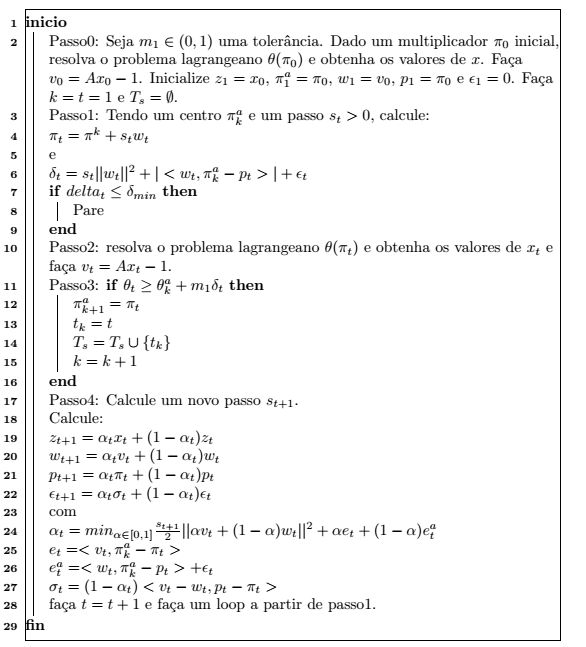
\includegraphics[width=4in]{AlgoritmoVolume.PNG}
\caption{Algoritmo do método do volume revisado para o problema lagrangeano $ \theta (\pi)$}
\label{AlgoritmoVolume}
\end{figure}